\documentclass[a4paper,10pt]{article}

\usepackage{adjustbox}
\usepackage{graphicx}
\usepackage{hyperref}
\usepackage{minted}
\usepackage{amsmath}
\usepackage{nbaseprt}
\usepackage[backend=biber,style=numeric,citestyle=numeric]{biblatex}

\bibliography{resources}

%opening
\title{The Memory \& Storage Design of Neo4J}
\author{Fabian Klopfer}

\begin{document}

\maketitle
\vspace{2cm}

\begin{abstract}
In this document I describe the internals of the storage layer of the popular native graph database Neo4J. 
    A detailed description of how records are stored into which files and how these are accessed is to be elaborated on in the following article.
    This is a translation, update and extension of previous work done by Michael Brendle. 
    Further the page cache (or buffer manager) and examples on access patterns generated by graph traversals are given. 
    This is done in order to gain insights and prepare for optimizing locality on the storage level to minimize IO\@.
\end{abstract} \newpage

\tableofcontents \newpage

\section{Introduction}
    \subsection{Database architecture}
        Relational databases store tables of data.
        The links considered in this category of DBMS are mostly used to stitch together the fields of an entry into one row again, after it has been split to satisfy a certain normal form.
        Of course one may also store tables where one table stores nodes and the other table's fields are node IDs to represent relationships.

        However, in order to traverse the graph, one has either to do a lot of rather expensive look ups or store auxiliary structures to speed up the look up process.
        In particular when using B-trees as index structure, each look up takes $\mathcal{O}(\log(n))$ steps to locate a specific edge.
        Alternatively one could store an additional table that holds edge lists such that the look up of outgoing or incomming edges is only $\mathcal{O}(\log(n))$ which would speed up breadth first traversals.
        But still one has to compute joins in order to continue the traversal in terms of depth.
        Another way to speed things up is to use a hash-based index, but this also has a certain overhead aside from the joins.

        In contrast to relational data base management systems, native graph data\-bases use structures specialised for this kind of queries.
        In the remainder of the document I discuss based upon Michael Brendle's work what structures and mechanisms the graph database Neo4J uses in order to achieve this superior performance in the domain of graphs.

        First of all, let us consider the high level architecture of a database management systems as shown in figure~\ref{dbms_arch} --- with a focus on the storage and loading elements.

        \begin{figure}[htp]\label{dbms_arch}
        \begin{center}
        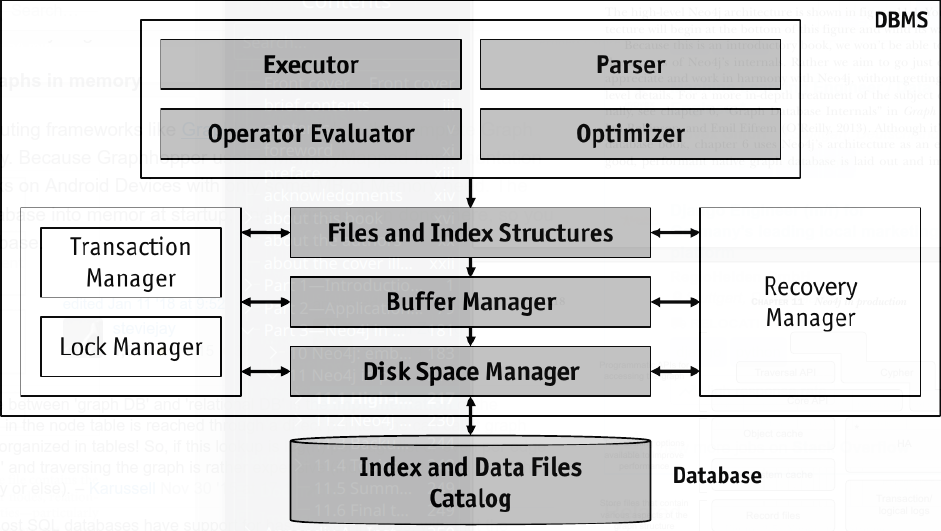
\includegraphics[keepaspectratio,width=0.7\textwidth]{img/00_intro/RDBMS.png}
        \end{center}
        \caption{The typical structure of a relational database management system.} %TODO citation
        \end{figure}

        Here The disk space manager, sometimes also called storage manager, handles de-/allocations, reads \& writes and provides the concept of a page: A disk block brought into memory. 
        For that it needs to keep track of free blocks in the allocated file. Optimally both a disk block and a page are of the same size. 
        One crucial task of a disk space manager is to store sequences of pages into continuous memory blocks in order to optimize data locality.
        Data locality has the upside, that one needs only one I/O operation to load multiple pages.
        To summarize the two most important objectives of a storage manager are to provide a locality-preserving mapping from pages to blocks based upon the information in the DBMS and to abstract physical storage to pages, taking care of allocation and access.
        A buffer manager is used to mediate between external storage and main memory. It maintains a designated pre-allocated area of main memory --- called the buffer pool --- to load, cache and evict pages into or from main memory.
        It's objective is to minimize the number of disk reads to be executed by caching, pre-fetching and the usage of suitable replacement policies. 
        It also needs to take care of allocating a certain fraction of pages to each transaction.

        \begin{figure}[htp]\label{dbms_memory}
            \begin{center}
            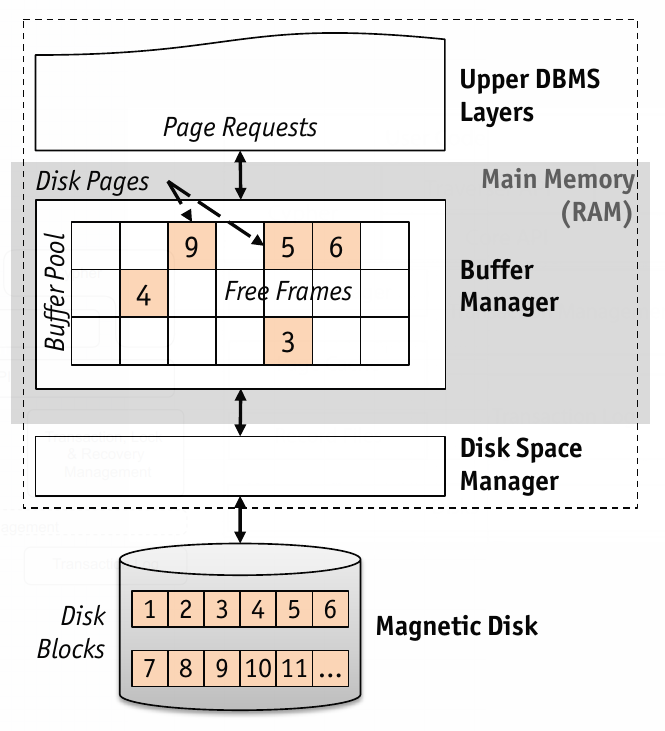
\includegraphics[keepaspectratio,height=0.4\textheight,width=0.5\textwidth]{img/00_intro/RDBMS_memory_view.png}
            \end{center}
            \caption{A visualization of the interaction of a database with memory.} %TODO citation
        \end{figure}

        The final memory and storage model relevant component of the  of a database management system is the file layout and possible index structures. 
        In order to store data a DBMS may either store one single or multiple files to maintain records. 

        A file may consist of a set of pages containing a set of slots. A slot stores one record with each record containing a set of fields. Further the database needs to keep track of free space in the file: A linked list or a directory must record free pages and some structure needs to keep track of the free slots either globally or per page. 

        Records may be of fixed or of variable size, depending on the types of their fields. 
        Records can be layout in row or column major order.
        That is one can store sequences of tuples or sequences of fields.
        The former is beneficial if a lot of update, insert or delete operations are committed to the database, while the latter optimizes the performance when scans and aggregations are the most typical queries to the system.

        Another option is to store the structure of the records along with pointers to the values of their fields in one files and the actual values in one or multiple separate files. 
        Also distinct types of tables can be stored in different files. 
        For example entities and relations can be stored in different files with references to each other, thus enabling the layout of these two to be specialized to their structure and usage in queries.

        Files may either organize their records in random order (heap file), sorted or using a hash function on one or more fields. 
        All of these approaches have upsides and downsides when it comes to scans, searches, insertions, deletions and updates. 

        To mitigate the effect that result from selecting one file organization or another, the concept of indexes have been introduced. 
        Indexes are auxiliary structures to speed up certain operations that depend on one field. 
        Indexes may be clustered or unclustered. 
        An index over field $F$ is called clustered if the underlying data file is sorted according to the values of $F$. 
        An unclustered index over field $G$ is one where the file is not sorted according to $G$. 
        In a similar way indexes can be sparse or dense. 
        A sparse index has less index entries than records, mostly one index entry per file. 
        This can of course only be done for clustered indexes as the sorting of the data file keeps the elements between index keys in order. 
        An index is dense if there is a one to one correspondence between records and index entries. 
        There are different variants of storing index entries which have again certain implications on the compactness of the index and the underlying design decisions.

        In another view of database management systems architectures, this boils down to the design decisions one has to make when implementing the storage layer and the access layer as shown in figure~\ref{dbms_arch_layers}.

        \begin{figure}[htp]\label{dbms_arch_layers}
        \begin{center}
        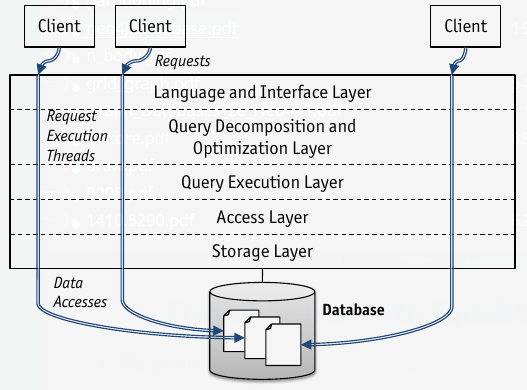
\includegraphics[keepaspectratio,width=0.6\textwidth]{img/00_intro/layered_RDBMS.png}
        \end{center}
        \caption{The architecture of a database management system from another point of view.} %TODO citation
        \end{figure}

        Here the storage layer is in close correspondence to the disk space manager in combination with the buffer manager, while the files and index structures provide the access layer.

        All these considerations make choosing different file splits, layouts, orderings, addressing schemes, management structures, de-/allocation schemes and indexes a complex set of dependent choices. 
        These depend mainly on the structure of the data to be stored and the queries to be run. 

    \subsection{The Architecture of Neo4J}
        When restricting to graph structures where nodes and relationships are allowed to have properties and labels and types respectively, this allows one to narrow down some of the design decisions.
        In particular the example of a popular graph native database --- Neo4J --- is what I discuss in the next sections. 

        To get an overview of the architecture let us consider figure~\ref{N4J_HLA_Emil}. 

        \begin{figure}[htp]\label{N4J_HLA_Emil}
        \begin{center}
        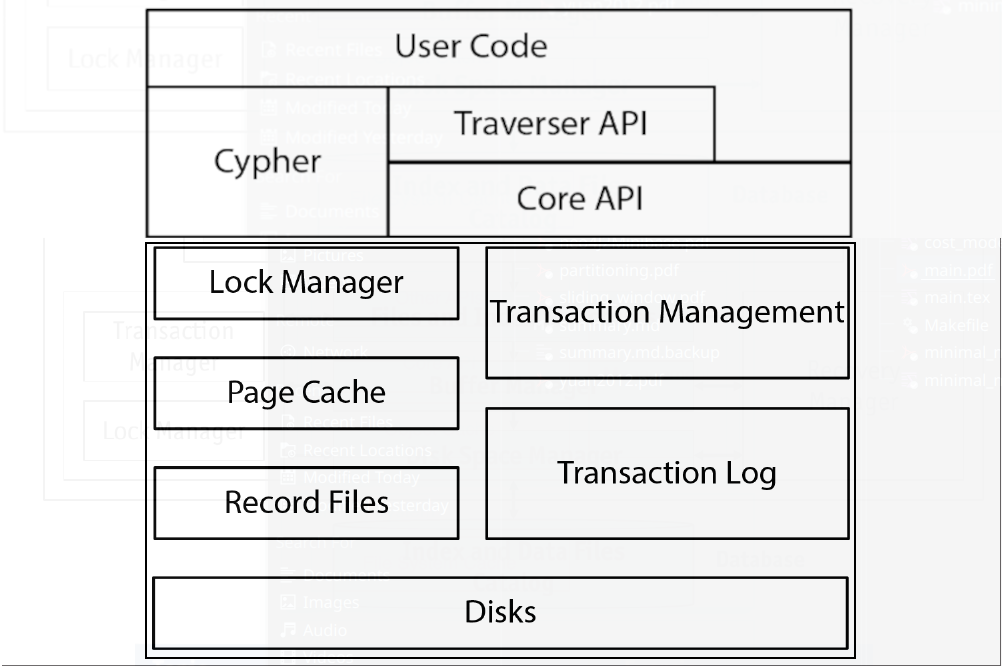
\includegraphics[keepaspectratio,width=0.6\textwidth]{img/00_intro/N4J_HLA_Emil.png}
        \end{center}
        \caption{The high level architecture of Neo4J according to Emil Efrim, the co-founder of Neo technologies.} %TODO citation
        \end{figure}

        Here we can see that the previous schema is not exactly straight forward to apply, mainly due to a lack of concise documentation.
        The diagram was taken from the only publication that elaborates on the internals of Neo4J aside from the code of course.
        Here The storage manager makes mostly use of the Java NIO package with some additional usage of operating system native calls to allocate memory for the page cache and network buffers. 
        A more detailed view on the high level architecture of the disk space and buffer manager and the files and index structures was deduced by the author from the source code and the non-public JavaDocs.
        This is shown in figure~\ref{N4J_Storage}.

        \begin{figure}[htp]\label{N4J_Storage}
        \begin{center}
        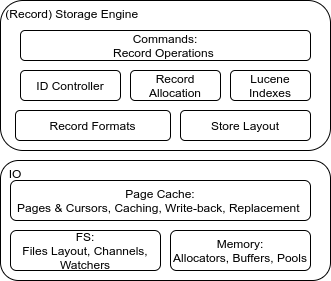
\includegraphics[keepaspectratio,width=0.5\textwidth]{img/00_intro/N4J_Storage.png}
        \end{center}
        \caption{A visualization of the broad the storage and memory organization of Neo4J.} %TODO citation
        \end{figure}

        In the next section the focus is set on the storage layer of Neo4J\@: How it handles allocations, read and writes and how it provides the notion of a page.
        After that I elaborate on the details of the page cache, the transformation it applies to nodes and relationships on loading, the caching and the page eviction strategies it employs.
        Finally the internals of the files and records layouts are discussed along with the special structures employed and the indexes that are (or may be) created over the files.

        The overall memory and storage state of a Neo4J instance and its environment may thus be visualized like this figure~\ref{N4J_memory_view}.

        \begin{figure}[htp]\label{N4J_memory_view}
        \begin{center}
        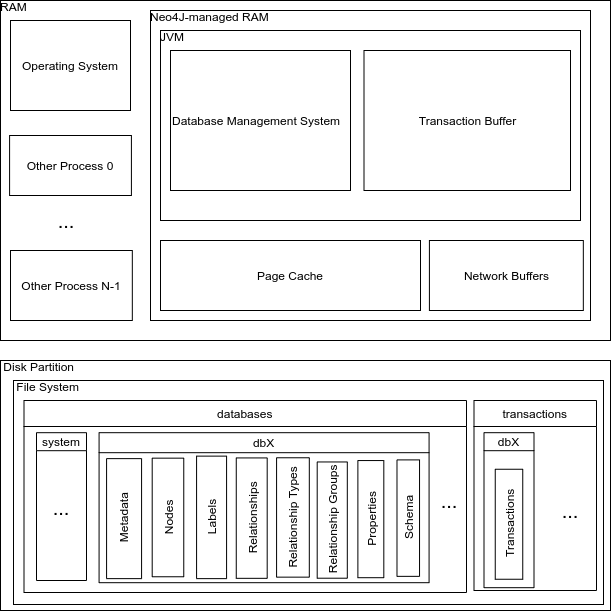
\includegraphics[keepaspectratio,width=\textwidth]{img/00_intro/N4J_memory_view.png}
        \end{center}
        \caption{A sketch of how Neo4J occupies memory.} %TODO citation
        \end{figure}

    \subsection{The Property Graph Model}
A \textbf{Property Graph} is a 9-Tuple $G = (V, E, \lambda, P, T, L, f_P, f_T, f_L)$ with 
\begin{itemize}
    \item $V$ the set of vertices.
    \item $E$ the set of edges.
    \item $\lambda: (V \times V) \rightarrow E$ a function assigning a pair of nodes to an edge.
    \item $L$ a set of strings used as labels.
    \item $P$ a set of key-value pairs called properties.
    \item $T$ a set of strings used as relationship types.
    \item $f_P: V \cup E \rightarrow 2^P$ a function that assigns a set of properties to a node or relationship.
   \item $f_T: E \rightarrow T$ a function that assigns a type to  a relationship.
   \item  $f_L: V \rightarrow 2^L$ a function that assigns a node a set of labels.
\end{itemize} 
\smallskip
The property graph model reflects a directed, node-labeled and relationship-typed multi-graph $G$, where each node and relationship can hold a set of key-value pairs~\autocite{angles2018property}. \\
    In a graph the edges are normally defined as $E \subseteq (V \times V)$, but in the property graph model edges have sets of properties and a type, which makes them objects on their own.
    An illustration of this model is shown in \ref{fig:propertygraph}
            \begin{figure}[htp]\label{fig:propertygraph}
        \begin{center}
        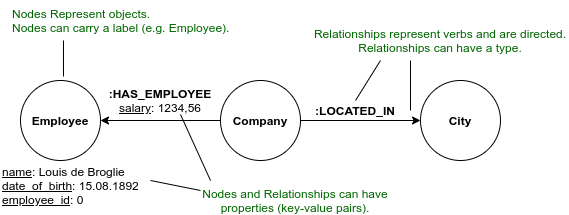
\includegraphics[keepaspectratio,width=\textwidth]{img/property_graph_elements.png}
        \end{center}
        \caption{A visualization of the property graph model.} %TODO citation
        \end{figure}
Neo4j is a graph database employing the property graph model~\cite{robinson2013graph}, which is used in the evaluation part of this thesis.


\newpage

\section{Disk Space \& Buffer Management}
    Neo4j uses a file for each record type. For each of these record files there exists another file that contains the IDs that are currently in use. Instead of Pages the database relies on Cursors. A cursor is a pointer to a location in a file that is to be loaded into a memory frame. Thus in order to load a record, the cursor is either moved within the file or a new cursor is opened and mapped to a frame. That means that a frame-sized window into the file is read. If a cursor is moved, it means that another frame-sized window is read and the former one is discarded.
    A positive side effect of that is that records do not have to be aligned to page boundaries in a strict sense. On the other hand it may occur that a half record is read, if the record size is not evenly divisable by the size of a frame.
    In contrast to earlier versions of Neo4j, records are loaded as they are and are not transformed into another representation.
    As pages do in other databases, cursors take care of reading and writing on the byte level. Finally the page cache in Neo4J uses a LRU scheduling policy to decide which cursors to replace by a new one. 
    \newpage
 

\section{File, Record \& Index Structures}\label{structure}
    \subsection{File Layout}\label{files_sec}
        The files that Neo4J uses to store data are categorizable into 5 classes based upon the records they contain:
        \begin{itemize}
            \item Node-related files: These files start with the prefixes \mintinline{bash}{neostore.nodestore*} and \mintinline{bash}{neostore.label*}. 
                The contents of these files contain the node structure and labels. 
            \item Relationship-related files: The prefix \mintinline{bash}{neostore.relationship*} is used for all files containing records related to the graph's relationship structure, types and possibly groups.
            \item Property-related files: Containing the properties of both nodes and relationship, this is the part that is least structured and rather unspecialized with respect to graphs.
            \item Schema: Files starting with \mintinline{bash}{neostore.schemastore*} contain information about the schema of the graph or rather the schematic information on the node, relationship and property labels, types and constraints.
            \item Metadata: Files only starting with \mintinline{bash}{neostore} and none of the above prefixes contain meta information about the graph.
            \item Finally, a lock file.
        \end{itemize}
        
        \begin{figure}[htp]\label{files}
            \begin{center}
                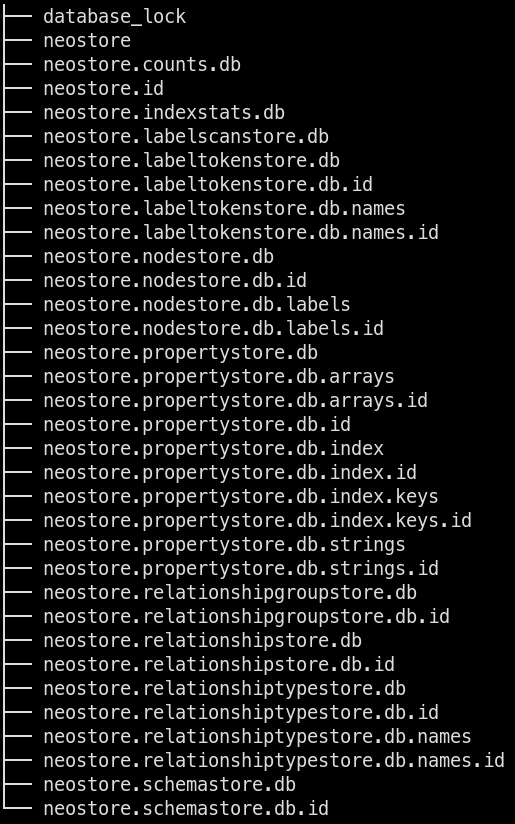
\includegraphics[keepaspectratio,height=0.4\textheight,width=0.5\textwidth]{img/03_record/files.png}
            \end{center}
            \caption{A visualization of the files layout of Neo4j.} 
        \end{figure}

        Most importantly the files ending with \mintinline{bash}{.db} contain all fixed size records representing the structure of the graph and small amounts of data.
        Files ending with \mintinline{bash}{.id} are used for record allocation and contain unused IDs. 
        Files having one of the suffixes \mintinline{bash}{names}, \mintinline{bash}{arrays} and \mintinline{bash}{strings} are so called dynamic stores and contain dynamic sized records. 
        A dynamic store is always started with a header block containing extra information and the offset to the first block in the store files. 
        Files ending with \mintinline{bash}{.index} contain indexes either generated by Neo4J (e.g.\ the keys of properties are referenced like this to avoid storing key names multiple times) or by the Apache Lucene indexing library.
        
    
    \subsection{Record Structures}
        \subsubsection{Address Translation}
            Neo4j defines the following constants as the size of the addresses used.
            \begin{figure}[htp]\label{addrsize}
                \adjustbox{varwidth=\textwidth, scale=0.9}{%
                    \inputminted{Java}{code/MaxIdLength.java}
                }
            \end{figure}
            These are represented by the datatype \mintinline{java}{long} when loaded into main memory. 
            On disk these values are stored as 32-bit \mintinline{java}{Integer}s with additional modifiers, that is the highest bits that do not fit into an int are stored to fields with additional space.
            
            For example the in-use bit consumes one byte of memory and the additional 7 bytes are used to stroe the highest bits that do not fit into an integer of another field.
            
            Finally the base and the modifer are aggregated into a long by shifting both appropriately, casting them to longs and applying the logical or \mintinline{java}{|} operation.
            
            Thus when refering to high bits and ID below, high bits do always mean the remainer of the bits that did not fit into the field that is said to be holding the ID\@.
            The latter is actually only holding the lowest 32 bits of an ID/address. The \textit{actual ID} is always high bits and ID field, shifted appropriately and connected using the logical or operator.
            
        \subsubsection{Nodes}
            The record format of nodes consist of a 15 byte structure.
            The IDs of nodes are stored implicitly as their address.
            If a node has ID 100 we know that its record starts at offset $15 \text{ Bytes} \cdot 100 = 1500$ from the beginning of the file.
            The struct of a record looks like this:
            \begin{enumerate}
                \item Byte 1: The first byte contains one bit for the in-use flag. 
                    The additional 7 bits are used to store the 3 highest bits of the relationship ID and the 4 highest bits of a property ID\@.
                \item Bytes 2 --- 5: The next 4 Bytes represent the ID of the first relationship in the linked list containing the relationships of the considered node.
                \item Bytes 6 --- 9: Again 4 bytes encode the ID to the first property of the node.
                \item Bytes 10 --- 14: This 5 byte section points to the labels of this node.
                \item Byte 15: The last byte stores if the node is dense, i.e.\ one node has an aweful lot of relationships and is treated a bit differently.
                    That is a relationships are stored by type and direction for this node into groups, see~\ref{rel_group}.
            \end{enumerate}
        
            \begin{figure}[htp]\label{node_record}
                \begin{center}
                    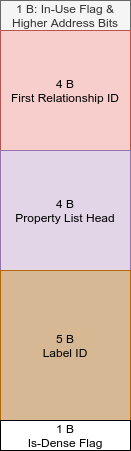
\includegraphics[keepaspectratio,height=0.4\textheight,width=0.5\textwidth]{img/03_record/node/node_record.png}
                \end{center}
                \caption{A visualization of the record structure of a node.}
            \end{figure}
            
            To summarize: The records on disk are stored as in the enumeration above. 
            In the database all IDs get mapped to longs and their respective space is larger than the space representable by 35 bit --- what is perfectly fine.
        
            \begin{figure}[htp]\label{node_first_byte}
                \begin{center}
                    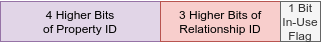
\includegraphics[keepaspectratio,height=0.4\textheight,width=0.5\textwidth]{img/03_record/node/node_first_byte.png}
                \end{center}
                \caption{A visualization of the information stored in the first byte of a node record.}
            \end{figure}
        
            On disk 4 byte integers are used to store the 32 lowest bits of the respective addresses and the higher bits are stored in the first byte that also carries the in-use bit.
        
          \paragraph{Node Labels}
            Each node label record consists of an in use bit and a name ID, which in turn points to an entry in a seperate file storing label names as dynamic records (see~\ref{dynamic}), storing the label names.
            This is done in order to assure that the records are of fixed length.
            \begin{enumerate}
                \item Byte 1: In-use flag
                \item Bytes 2 --- 5: Pointer to the label string entry
            \end{enumerate}
            
            \begin{figure}[htp]\label{label_record}
                \begin{center}
                    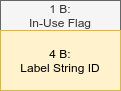
\includegraphics[keepaspectratio,height=0.2\textheight,width=0.2\textwidth]{img/03_record/node/label_record.png}
                \end{center}
                \caption{A visualization of the structure of a label record.}
            \end{figure}
            
            
        
        \subsubsection{Relationships}
            \begin{figure}[htp]\label{rel_record}
                \begin{center}
                    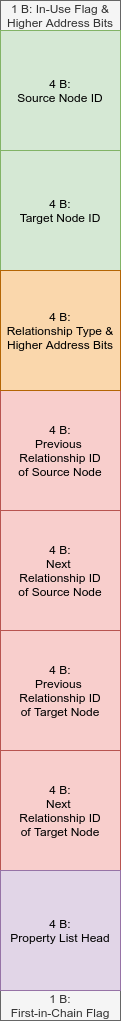
\includegraphics[keepaspectratio,height=0.9\textheight,width=0.5\textwidth]{img/03_record/relationship/relationship_record.png}
                \end{center}
                \caption{A visualization of the record structure of a relationship in Neo4J.} 
            \end{figure}
            
            Relationship records are stored with implicit IDs too. 
            Their fixed size records contain 34 bytes.
            Besides an in-use flag and the node IDs that are connected, and the relationship type, the record also contains two doubly linked list: One for the relationships of the first node and one for the relationship of the second node.
            Finally a link to the head of the properties linked list of this relationship and a marker if this relationship is the first element in the relationships linked list of one of the nodes.
            \newpage
            
            \begin{enumerate}
                \item Byte 1: In-use bit, first node high order bits (3 bits), first property high order bits (4 bits)
                \item Bytes 2 --- 5: first node ID 
                \item Bytes 6 --- 9: second node ID 
                \item Bytes 10 --- 13: relationship type (16 bit), second node high order bits (3 bits), relationship previous and next ID higher bits for first and second node ($4 \cdot 3 = 12$ bits), one unused bit.
                \item Bytes 14 --- 17: previous relationship ID for first node
                \item Bytes 18 --- 21: next relationship ID for first node
                \item Bytes 22 --- 25: previous relationship ID for second node
                \item Bytes 26 --- 29: next relationship ID for second node
                \item Bytes 30 --- 33: link to the first property of the relationship
                \item Bytes 34: A marker if this relation is the first element in the relationship linked list of one of the nodes stored in the lowest two bits of the byte. 
                    The other 6 bits are unused.
            \end{enumerate}


            \begin{figure}[htp]\label{rel_first_byte}
                \begin{center}
                    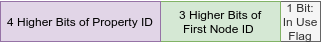
\includegraphics[keepaspectratio,width=\textwidth]{img/03_record/relationship/relationship_first_byte.png}
                \end{center}
                \caption{A visualization of how information is stored in the first byte of a relationship record.} 
            \end{figure}

            \begin{figure}[htp]\label{rel_type_bytes}
                \begin{center}
                    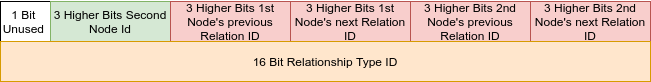
\includegraphics[keepaspectratio,width=\textwidth]{img/03_record/relationship/relationship_type_bytes.png}
                \end{center}
                \caption{The structure of the bytes that are used to store the type of a relationship and high bits of a node and a relationship IDs.}
            \end{figure}
        

        \subsubsection{Relationship Types}
            Similarly to the node labels, the relationship type records posses an in-use flag and a type ID that points to a record in a file containing strings in the dynamic record format.
            \begin{enumerate}
                \item Byte 1: In-use flag
                \item Bytes 2 --- 5: Pointer to the type string entry
            \end{enumerate}
        
            \begin{figure}[htp]\label{rel_type_record}
                \begin{center}
                    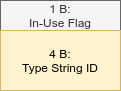
\includegraphics[keepaspectratio,height=0.2\textheight,width=0.2\textwidth]{img/03_record/relationship/rel_type_record.png}
                \end{center}
                \caption{A visualization of the record structure of a relationship type.} 
            \end{figure}
            
        \subsubsection{Relationship Groups}~\label{rel_group}
            The relationship group record is used for dense nodes in order not to iterate over all relationships but only over those of a specific type.
            Each record consists of 25 bytes where the first byte again contains the in-use flags and the high order bits of IDs that do not fit into integers.
            The next bytes again contains high bits of addresses and is followed by the relationship type.
            After that a reference (an ID) to the next relationship group record is given.
            Finally the first outgoing relation, the first incoming relation, the first looping relation and the node of interest are specified.
        
            \begin{figure}[htp]\label{rel_group_record}
                \begin{center}
                    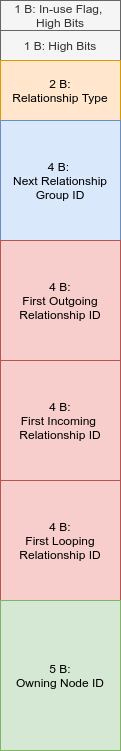
\includegraphics[keepaspectratio,height=0.2\textheight,width=0.2\textwidth]{img/03_record/relationship/relationship_group_record.png}
                \end{center}
                \caption{A visualization of the record structure of a relationship group.}
            \end{figure}
        
            \begin{enumerate}
                \item Byte 1: In-use flag, high bits for the next relationship group ID, high bits for the first entry of outgoing relationship list.
                \item Byte 2: High bits for the first entry in the incoming relationship list, high bits for the first entry in the looping relationship list.
                \item Bytes 3 and 4: Relationship type ID
                \item Bytes 5 --- 8: ID of the next relationship group record.
                \item Bytes 9 --- 12: ID of the first relationship in the linked list of outgoing relationships, i.e.\ those relationships which start at the record owning node.
                \item Bytes 13 --- 16: ID of the first relationship in the linked list of incoming relationships, i.e.\ those relationships which end at the record owning node.
                \item Bytes 17 --- 20: ID of the first relationship in the linked list of loops, i.e.\ relationships which start and end at the record owning node.
                \item Bytes 21 --- 25: ID of the node for which the relationship group was created, also called the owning node (in the source code).
            \end{enumerate}
            
            \begin{figure}[htp]\label{rel_group_first_bytes}
                \begin{center}
                    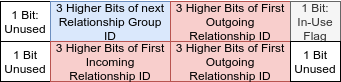
\includegraphics[keepaspectratio,height=0.2\textheight,width=0.2\textwidth]{img/03_record/relationship/relationship_group_first_bytes.png}
                \end{center}
                \caption{The structure of the first two bytes of a relationship group record.}
            \end{figure}
        

        \subsubsection{Properties}
            Properties are stored per node or relationship as doubly linked list of 41 byte records with the first 9 bytes storing the previous and next property IDs and the remaining 32 bytes carry so called property blocks.
            \begin{enumerate}
            \item Byte 1: High bits of next and previous property IDs
            \item Bytes 2 --- 5: Previous property ID
            \item Bytes 6 --- 9: Next property ID
            \item Bytes 10 --- 41: Up to 4 Property Blocks
            \end{enumerate}
            
            \begin{figure}[htp]\label{prop}
                \begin{center}
                    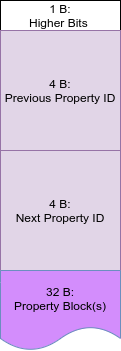
\includegraphics[keepaspectratio,height=0.2\textheight,width=0.2\textwidth]{img/03_record/property/property.png}
                \end{center}
                \caption{The structure of a property record.}
            \end{figure}
            
          \paragraph{Property Blocks} 
            Each propety block consists of one to four 8 byte value blocks.
            Thus each property block spans between 8 and 32 byte.
            The first value block of a property block has the following structure:
            \begin{enumerate}
                \item Byte 1 --- 3: Property key index ID (pointer to the key name)
                \item Byte 4: Type, inlined flag and 3 bits data
                \item Byte 5 --- 8: Data
            \end{enumerate}
            \textit{TODO correct figure to have lsb and msb inverted, inlined flag needs to be on the ´´surface'' instead of the inside.} \\
            
            At least this order would feel natural (first the header then data).
            However the engineers at Neo Technologies have decided to swap the endianness of a property block.
            In order to complete the confusion, they use a special encoding derived from the Latin 1 encoding for all in-lined types which is described in \mintinline[fontsize=\tiny]{bash}{neo4j/community/record-storage-engine/src/main/java/org/neo4j/kernel/impl/store/LongerShortString.java}.
            The decoding step is implemented from line 900 to line 1000.
            The coding tables are implemented from lines 30 too 600.
            
            \begin{figure}[htp]\label{prop_block}
                \begin{center}
                    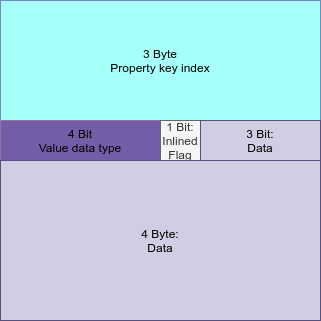
\includegraphics[keepaspectratio,height=0.2\textheight,width=0.2\textwidth]{img/03_record/property/property_block.png}
                \end{center}
                \caption{The structure of a property block.}
            \end{figure}
            
            All remaining value blocks contain pure data. 
            Property values of type boolean, byte, short, int, char and float fit into one property block with one value block. 
            Properties of type long and double are stored into two value blocks. 
            Short strings and arrays are stored in the same property block as well, if they fit into 28 byte.
            Otherwise a reference is stored, that refers to one of the respective dynamic stores for array and string property values. 
            Other types such as temporal and spatial data are also fit into one property block. 
            Details on each data type are outlined in the comment from the source code shown below. 
            As there are only 14 different types, 4 bits suffice to encode the type. 
            The types are enumerated in the order given below starting at \mintinline{java}{0b0001}. \\
            
            \textit{TODO requires further elaboration on in-lined values}
            
            \begin{figure}[htp]\label{property_types}
                \begin{center}    
                    \adjustbox{varwidth=\textwidth}{%
                        \inputminted{Java}{code/PropertyTypeEnum.java}
                    }
                \end{center}
                \caption{The type enumeration used for property blocks}
            \end{figure}
            
            \begin{figure}[htp]\label{property_Value_formats}
                \begin{center}
                    \adjustbox{varwidth=\textwidth, scale=0.9}{%
                        \inputminted[autogobble, fontsize=\scriptsize]{java}{code/PropertyTypeLayout.java}
                    }
                \end{center}
                \caption{The layout of different types in property blocks.}
            \end{figure}
            
          \paragraph{Property Key Index}
            The property key index contains a in-use flag, a usage count and a reference to the respective name string in a dynamic store.
            \begin{enumerate}
            \item Byte 1: In-use Flag
            \item Byte 2 --- 5: 
            \end{enumerate}
                \begin{figure}[htp]\label{prop_key_idx}
                \begin{center}
                    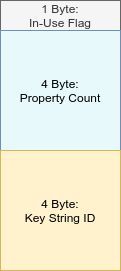
\includegraphics[keepaspectratio,height=0.2\textheight,width=0.2\textwidth]{img/03_record/property/property_key_index.png}
                \end{center}
                \caption{The structure of a property key index record.}
            \end{figure}

            
        \subsubsection{Dynamic Records: Strings \& Arrays}\label{dynamic}
            \begin{figure}[htp]\label{dynamic_rec}
                \begin{center}
                    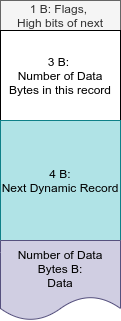
\includegraphics[keepaspectratio,height=0.2\textheight,width=0.2\textwidth]{img/03_record/dynamic.png}
                \end{center}
                \caption{The structure of a dynamic record.} 
            \end{figure}
            A record in a dynamic store is either strings or arrays stored as properties,  the strings of node labels or relationship types each of which stored in their own dynamic store.
            A dynamic record has 8 fixed bytes followed by up to $2^{24}$ bytes $= 16 $MiB.
            If the string or array to be stored is larger, then the remainder of the data is stored using a linked list of next blocks.
            The absolute amount of dynamic data that can be stored that way is only limited by the machines disk space, so potentially infinite (as the admin could keep on buying new disks). 
            The structure of such a record is as follows:
            \begin{enumerate}
                \item 1 Byte: Start or linked record flag, in-use flag, high bits of next block ID
                \item 2 --- 4: Number of bytes used to store data beginning after the header.
                \item 5 --- 8: Reference to the next dynamic record
                \item 9 --- Number of bytes used $- 1$: Data
            \end{enumerate}
            
            \begin{figure}[htp]\label{dynamic_first}
                \begin{center}
                    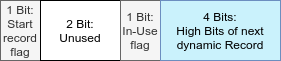
\includegraphics[keepaspectratio,height=0.2\textheight,width=0.2\textwidth]{img/03_record/dynamic_first_byte.png}
                \end{center}
                \caption{The first byte of a dynamic record.}
            \end{figure}

                            
        \subsection{Record Allocation}
            TODO later \\
            \href{https://neo4j.com/docs/operations-manual/current/performance/space-reuse/\#space-reuse}{Reusing space} \\
            \href{https://neo4j.com/developer/kb/how-deletes-workin-neo4j/}{How delete works} \\
        
\section{Examples}
    First we give an example graph in the visual form. A simple social network that is created using the Cypher query shown in figure~\ref{ex_q}
    \begin{figure}[htp]\label{ex_q}
        \begin{center}
            \inputminted{Cypher}{code/example_query.cy}
        \end{center}
        \caption{The Cypher query to generate the example visualized below.}
    \end{figure}
    This graph is visualized by Neo4J with what is shown in figure~\ref{graph}. As we can see we have four nodes and five edges. The edges are directed. The graph represents who knows whom with respect to the four nodes representing users.
    \begin{figure}[htp]\label{graph}
        \begin{center}
            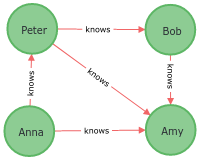
\includegraphics[keepaspectratio,height=0.3\textheight,width=0.3\textwidth]{img/04_example/graph.png}
        \end{center}
        \caption{The graph of the above cypher query visualized on a high level.} 
    \end{figure}
    
    In this figure, the focus is on how the graph is represented structurally. The bigger and wider red arrows and greenish circles are solely to aid with perception. The actual contents is held in the tables and thinner but bold arrows representing some of the structures elaborated on in the previous Section~\ref{structure}.
    Lets start with the nodes.
    Those are the 3 slot tables in the greenish circles.
    The red field points to the first relationship in that the node is involved. 
    The second field points to the first property record of the node. 
    The last field contains the node label which is in-lined in order not to use even more arrows than there are already.
    The relationship structure is more involved: The first two fields contain references to node from which the relationship originates and the node where the relationship ends.
    This is followed by a pointer to the corresponding relationship type, which is again in-lined here for visualisation purposes.
    The next four fields contain the previous and next elements of the linked list of relationships of the two nodes. 
    Finally in the last field is a reference to the first property of the relationship.\\
    \begin{figure}[htp]\label{example_structs}
        \begin{center}
            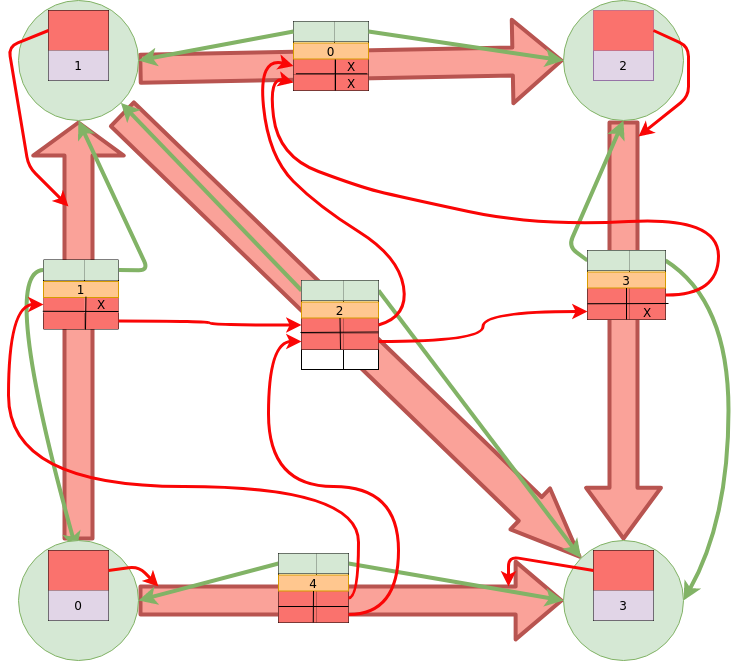
\includegraphics[keepaspectratio,height=1.2\textheight,width=1.2\textwidth]{img/04_example/example_structs.png}
        \end{center}
        \caption{The same graph as before, with additional conceptual information about its storage format.}
    \end{figure}
    
    As discussed in Subsection~\ref{files_sec}, the information is stored into different files. 
    The first part of these files holding the records of the above graph is shown in binary format in the figures~\ref{nodes},~\ref{label_tokens},~\ref{label_strings},~\ref{relationships},~\ref{relation_type_token},~\ref{relationship_type_string},~\ref{properties},~\ref{property_keys}
    \begin{figure}[htp]\label{nodes}
        \begin{center}
            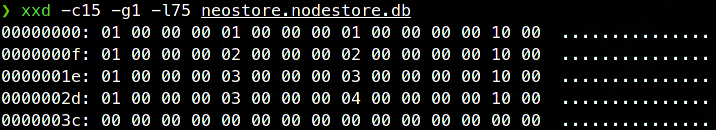
\includegraphics[keepaspectratio,height=1.2\textheight,width=1.2\textwidth]{img/04_example/nodes.png}
        \end{center}
        \caption{The nodes of the just presented graph.}
    \end{figure}
    \begin{figure}[htp]\label{label_tokens}
        \begin{center}
            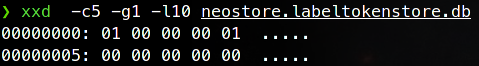
\includegraphics[keepaspectratio,height=1.2\textheight,width=1.2\textwidth]{img/04_example/label_token.png}
        \end{center}
        \caption{The label tokens as stored on disk.} 
    \end{figure}
    \begin{figure}[htp]\label{label_strings}
        \begin{center}
            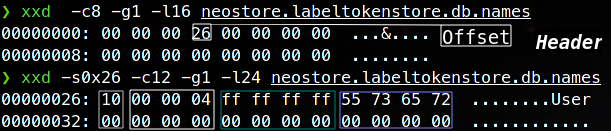
\includegraphics[keepaspectratio,height=1.2\textheight,width=1.2\textwidth]{img/04_example/labels_string_dynamic.png}
        \end{center}
        \caption{The label strings as persisted in the dynamic storage file.}
    \end{figure}
    \begin{figure}[htp]\label{relationships}
        \begin{center}
            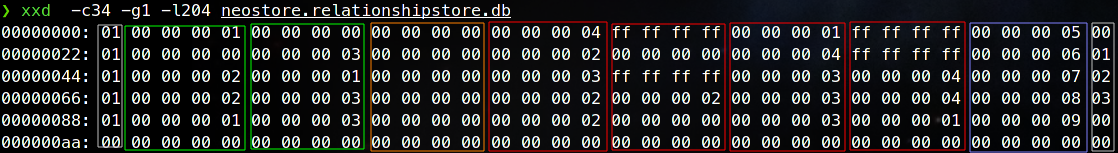
\includegraphics[keepaspectratio,height=1.2\textheight,width=1.2\textwidth]{img/04_example/relationships.png}
        \end{center}
        \caption{The relationship records of out example graph.}
    \end{figure}
    \begin{figure}[htp]\label{relation_type_token}
        \begin{center}
            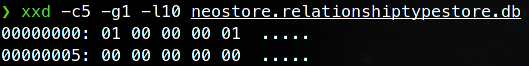
\includegraphics[keepaspectratio,height=1.2\textheight,width=1.2\textwidth]{img/04_example/relationshiptype_token.png}
        \end{center}
        \caption{The relationship type records.} 
    \end{figure}
    \begin{figure}[htp]\label{relationship_type_string}
        \begin{center}
            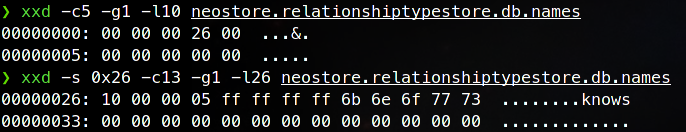
\includegraphics[keepaspectratio,height=1.2\textheight,width=1.2\textwidth]{img/04_example/relationshiptype_string_dynamic.png}
        \end{center}
        \caption{The relationship type strings stored in a dynamic store.} 
    \end{figure}
    \begin{figure}[htp]\label{properties}
        \begin{center}
            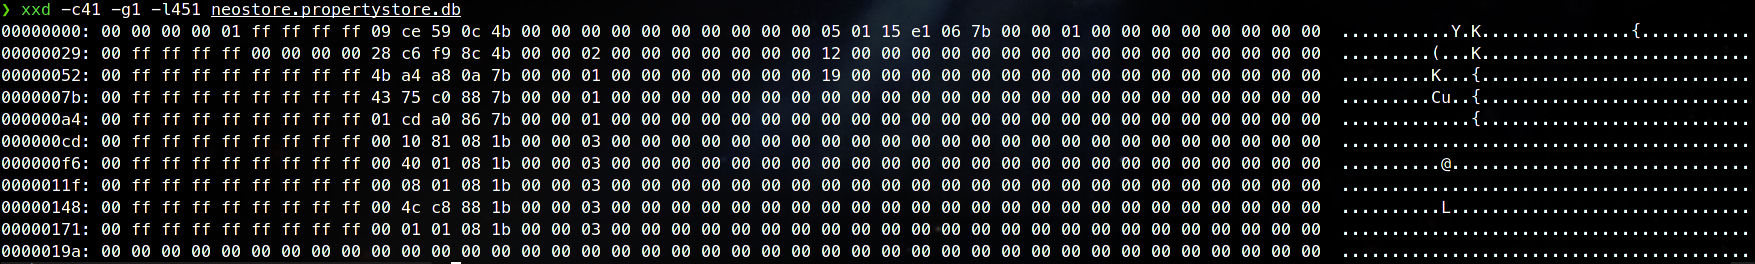
\includegraphics[keepaspectratio,height=1.2\textheight,width=1.2\textwidth]{img/04_example/properties.png}
        \end{center}
        \caption{The relationship records of out example graph.}
    \end{figure}
    \begin{figure}[htp]\label{property_keys}
        \begin{center}
            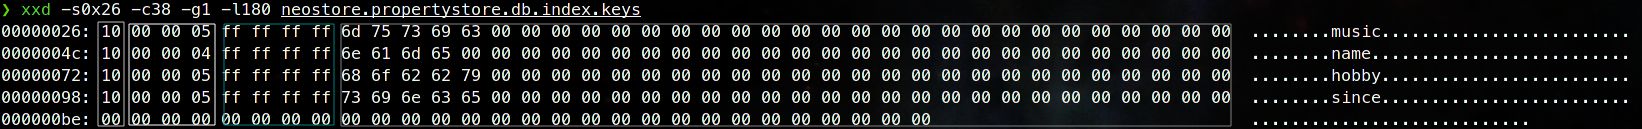
\includegraphics[keepaspectratio,height=1.2\textheight,width=1.2\textwidth]{img/04_example/property_key_strings.png}
        \end{center}
        \caption{The relationship records of out example graph.}
    \end{figure}
    
    \subsection{Purely disk-based Access}
        \subsubsection{BFS Traversal}
            Undirected BFS example: Starting at Anna, what's the shortest path to Bob? \\
            Traversal order:
            \begin{enumerate}
                \item Anna's node (node id 2, address \nbaseprint{0x1E}) $\rightarrow$ Reference to her first relationship (relationship id 3, address \nbaseprint{0x66}), followed by the link to the second relationship (relationship id 2, address \nbaseprint{0x44}). \\
             None of them is Bob already, so continue with the first relationships target and its arcs.
         \item The first target node was Amy (node ID 3, address \nbaseprint{0x2D}). Her first relationship is again relationship relationship id 3 (address \nbaseprint{0x66}) which needs to be accessed to retrieve the next element from her linked list.
             The second element in this list is relationship with ID 4 (address \nbaseprint{0x88}). 
                    The last relationship in her linked list has ID 01 (address \nbaseprint{0x11}) and is indeed one that has Bob as target node. 
                    Thus the search can be terminated and the so found path from Anna (node ID 2) via relationship with ID 3 to Amy (node ID 3) to Bob (node ID 0) using relationship ID 1 can be returned.
            \end{enumerate}
            What got rather obvious here is that the order of the nodes and relationship on disk is the insertion order.
            Here the graph was small and all nodes and relationships can easily fit on one page (standard size 4096 B). 
            But when the graph gets larger and the insertion order does not match paths, the accesses are effectively random. 
                       
            
\nocite{*}
\printbibliography{}

\end{document}
